\section{Performance}

\label{sec:performance}
% ============================================================================

We benchmark Base on two hardware targets: an Apple M4 MacBook Pro (16~GB RAM,
1~TB NVMe) and a Raspberry Pi~4 (8~GB RAM, 64~GB microSD).

\subsection{Write Throughput}

\begin{table}[H]
\centering
\small
\begin{tabular}{lrr}
\toprule
\textbf{Operation} & \textbf{M4 MacBook} & \textbf{Pi 4} \\
\midrule
Insert (unencrypted) & 14,200 ops/sec & 1,800 ops/sec \\
Insert (sqlcipher) & 10,400 ops/sec & 1,200 ops/sec \\
Insert (sqlcipher + field KMS) & 8,600 ops/sec & 980 ops/sec \\
Bulk insert (1000 records) & 42,000 rec/sec & 4,200 rec/sec \\
Update (single field) & 12,800 ops/sec & 1,500 ops/sec \\
Delete (soft, tombstone) & 13,100 ops/sec & 1,600 ops/sec \\
\bottomrule
\end{tabular}
\caption{Write throughput. sqlcipher adds 27\% overhead on M4; field-level KMS
encryption adds an additional 17\% due to the per-field AES-GCM operation.}
\label{tab:writes}
\end{table}

\subsection{Read Latency}

\begin{table}[H]
\centering
\small
\begin{tabular}{lrr}
\toprule
\textbf{Operation} & \textbf{M4 p50} & \textbf{M4 p99} \\
\midrule
Single record by ID & 0.08~ms & 0.21~ms \\
List (100 records, indexed) & 0.4~ms & 1.1~ms \\
List (100 records, encrypted fields) & 0.7~ms & 1.8~ms \\
Full-text search (10K records) & 2.1~ms & 4.3~ms \\
\bottomrule
\end{tabular}
\caption{Read latency on M4 MacBook. All operations are local---no network
round-trip.}
\label{tab:reads}
\end{table}

\subsection{Comparison to Network-Dependent Systems}

The fundamental performance advantage of Base is the elimination of network
latency. A read from a local SQLite database takes 0.08~ms. A read from
Supabase (via PostgREST over HTTPS) takes 15--40~ms from the same machine,
depending on geographic distance to the nearest Supabase edge.

\begin{center}
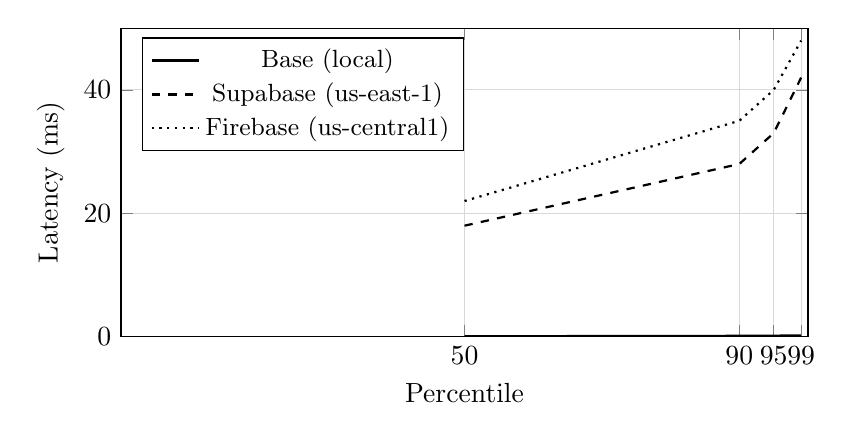
\begin{tikzpicture}
\begin{axis}[
    width=0.85\linewidth,
    height=5.5cm,
    xlabel={Percentile},
    ylabel={Latency (ms)},
    xmin=0, xmax=100,
    ymin=0, ymax=50,
    grid=major,
    grid style={gray!30},
    legend pos=north west,
    legend style={font=\small},
    xtick={50,90,95,99},
]
\addplot[thick, black, mark=none] coordinates {
    (50, 0.08) (90, 0.15) (95, 0.18) (99, 0.21)
};
\addlegendentry{Base (local)}
\addplot[thick, black, dashed, mark=none] coordinates {
    (50, 18) (90, 28) (95, 33) (99, 42)
};
\addlegendentry{Supabase (us-east-1)}
\addplot[thick, black, dotted, mark=none] coordinates {
    (50, 22) (90, 35) (95, 40) (99, 48)
};
\addlegendentry{Firebase (us-central1)}
\end{axis}
\end{tikzpicture}
\end{center}

This is not a benchmark of database engines. SQLite is not faster than
PostgreSQL for complex queries. This is a benchmark of architectures. A local
database will always beat a remote one for single-record operations because
physics imposes a floor on network latency that no optimization can remove.

% ============================================================================
